\documentclass[twoside]{book}

% Packages required by doxygen
\usepackage{fixltx2e}
\usepackage{calc}
\usepackage{doxygen}
\usepackage[export]{adjustbox} % also loads graphicx
\usepackage{graphicx}
\usepackage[utf8]{inputenc}
\usepackage{makeidx}
\usepackage{multicol}
\usepackage{multirow}
\PassOptionsToPackage{warn}{textcomp}
\usepackage{textcomp}
\usepackage[nointegrals]{wasysym}
\usepackage[table]{xcolor}

% Font selection
\usepackage[T1]{fontenc}
\usepackage[scaled=.90]{helvet}
\usepackage{courier}
\usepackage{amssymb}
\usepackage{sectsty}
\renewcommand{\familydefault}{\sfdefault}
\allsectionsfont{%
  \fontseries{bc}\selectfont%
  \color{darkgray}%
}
\renewcommand{\DoxyLabelFont}{%
  \fontseries{bc}\selectfont%
  \color{darkgray}%
}
\newcommand{\+}{\discretionary{\mbox{\scriptsize$\hookleftarrow$}}{}{}}

% Page & text layout
\usepackage{geometry}
\geometry{%
  a4paper,%
  top=2.5cm,%
  bottom=2.5cm,%
  left=2.5cm,%
  right=2.5cm%
}
\tolerance=750
\hfuzz=15pt
\hbadness=750
\setlength{\emergencystretch}{15pt}
\setlength{\parindent}{0cm}
\setlength{\parskip}{3ex plus 2ex minus 2ex}
\makeatletter
\renewcommand{\paragraph}{%
  \@startsection{paragraph}{4}{0ex}{-1.0ex}{1.0ex}{%
    \normalfont\normalsize\bfseries\SS@parafont%
  }%
}
\renewcommand{\subparagraph}{%
  \@startsection{subparagraph}{5}{0ex}{-1.0ex}{1.0ex}{%
    \normalfont\normalsize\bfseries\SS@subparafont%
  }%
}
\makeatother

% Headers & footers
\usepackage{fancyhdr}
\pagestyle{fancyplain}
\fancyhead[LE]{\fancyplain{}{\bfseries\thepage}}
\fancyhead[CE]{\fancyplain{}{}}
\fancyhead[RE]{\fancyplain{}{\bfseries\leftmark}}
\fancyhead[LO]{\fancyplain{}{\bfseries\rightmark}}
\fancyhead[CO]{\fancyplain{}{}}
\fancyhead[RO]{\fancyplain{}{\bfseries\thepage}}
\fancyfoot[LE]{\fancyplain{}{}}
\fancyfoot[CE]{\fancyplain{}{}}
\fancyfoot[RE]{\fancyplain{}{\bfseries\scriptsize Generated by Doxygen }}
\fancyfoot[LO]{\fancyplain{}{\bfseries\scriptsize Generated by Doxygen }}
\fancyfoot[CO]{\fancyplain{}{}}
\fancyfoot[RO]{\fancyplain{}{}}
\renewcommand{\footrulewidth}{0.4pt}
\renewcommand{\chaptermark}[1]{%
  \markboth{#1}{}%
}
\renewcommand{\sectionmark}[1]{%
  \markright{\thesection\ #1}%
}

% Indices & bibliography
\usepackage{natbib}
\usepackage[titles]{tocloft}
\setcounter{tocdepth}{3}
\setcounter{secnumdepth}{5}
\makeindex

% Hyperlinks (required, but should be loaded last)
\usepackage{ifpdf}
\ifpdf
  \usepackage[pdftex,pagebackref=true]{hyperref}
\else
  \usepackage[ps2pdf,pagebackref=true]{hyperref}
\fi
\hypersetup{%
  colorlinks=true,%
  linkcolor=blue,%
  citecolor=blue,%
  unicode%
}

% Custom commands
\newcommand{\clearemptydoublepage}{%
  \newpage{\pagestyle{empty}\cleardoublepage}%
}

\usepackage{caption}
\captionsetup{labelsep=space,justification=centering,font={bf},singlelinecheck=off,skip=4pt,position=top}

%===== C O N T E N T S =====

\begin{document}

% Titlepage & ToC
\hypersetup{pageanchor=false,
             bookmarksnumbered=true,
             pdfencoding=unicode
            }
\pagenumbering{roman}
\begin{titlepage}
\vspace*{7cm}
\begin{center}%
{\Large test }\\
\vspace*{1cm}
{\large Generated by Doxygen 1.8.11}\\
\end{center}
\end{titlepage}
\clearemptydoublepage
\tableofcontents
\clearemptydoublepage
\pagenumbering{arabic}
\hypersetup{pageanchor=true}

%--- Begin generated contents ---
\chapter{Todo List}
\label{todo}
\hypertarget{todo}{}

\begin{DoxyRefList}
\item[\label{todo__todo000002}%
\hypertarget{todo__todo000002}{}%
Global \hyperlink{proxy__cache_8c_aff2ddf6eae4259a4833bdef91a829f6c}{find\+\_\+primecache} (const char $\ast$path\+\_\+primecache, const char $\ast$hash\+\_\+full)]Implement the H\+IT case.  
\item[\label{todo__todo000001}%
\hypertarget{todo__todo000001}{}%
Global \hyperlink{proxy__cache_8c_a2e94ab3968ac908363e0ed7a6dcc3459}{find\+\_\+subcache} (const char $\ast$path\+\_\+subcache, const char $\ast$hash\+\_\+back)]Implement the H\+IT case. 
\end{DoxyRefList}
\chapter{File Index}
\section{File List}
Here is a list of all documented files with brief descriptions\+:\begin{DoxyCompactList}
\item\contentsline{section}{\hyperlink{proxy__cache_8c}{proxy\+\_\+cache.\+c} }{\pageref{proxy__cache_8c}}{}
\end{DoxyCompactList}

\chapter{File Documentation}
\hypertarget{proxy__cache_8c}{}\section{proxy\+\_\+cache.\+c File Reference}
\label{proxy__cache_8c}\index{proxy\+\_\+cache.\+c@{proxy\+\_\+cache.\+c}}
{\ttfamily \#include $<$dirent.\+h$>$}\\*
{\ttfamily \#include $<$errno.\+h$>$}\\*
{\ttfamily \#include $<$fcntl.\+h$>$}\\*
{\ttfamily \#include $<$pwd.\+h$>$}\\*
{\ttfamily \#include $<$stdio.\+h$>$}\\*
{\ttfamily \#include $<$stdlib.\+h$>$}\\*
{\ttfamily \#include $<$string.\+h$>$}\\*
{\ttfamily \#include $<$unistd.\+h$>$}\\*
{\ttfamily \#include $<$openssl/sha.\+h$>$}\\*
{\ttfamily \#include $<$sys/stat.\+h$>$}\\*
{\ttfamily \#include $<$sys/types.\+h$>$}\\*
Include dependency graph for proxy\+\_\+cache.\+c\+:\nopagebreak
\begin{figure}[H]
\begin{center}
\leavevmode
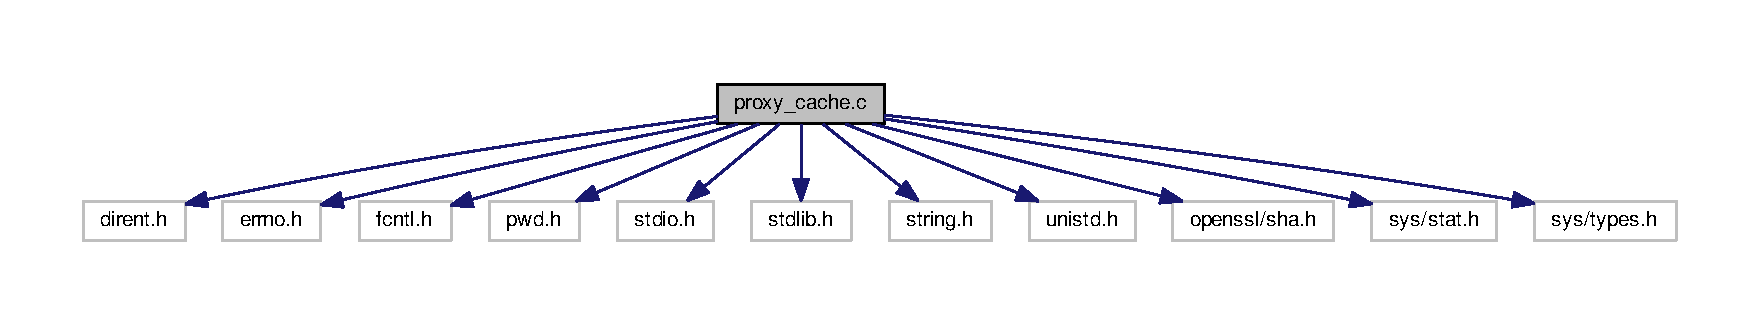
\includegraphics[width=350pt]{proxy__cache_8c__incl}
\end{center}
\end{figure}
\subsection*{Enumerations}
\begin{DoxyCompactItemize}
\item 
enum \hyperlink{proxy__cache_8c_a1e98c665f4a7e4770cbe6a5c54e8ff83}{P\+R\+O\+X\+Y\+\_\+\+C\+O\+N\+S\+T\+A\+N\+TS} \{ \hyperlink{proxy__cache_8c_a1e98c665f4a7e4770cbe6a5c54e8ff83ad9e994f11159cb207fcf2c88e2749f8b}{P\+R\+O\+X\+Y\+\_\+\+L\+E\+N\+\_\+\+P\+R\+E\+F\+IX} = 3, 
\hyperlink{proxy__cache_8c_a1e98c665f4a7e4770cbe6a5c54e8ff83af88ac79de02fd8c04aede21e1615340b}{P\+R\+O\+X\+Y\+\_\+\+L\+E\+N\+\_\+\+H\+A\+SH} = 41, 
\hyperlink{proxy__cache_8c_a1e98c665f4a7e4770cbe6a5c54e8ff83aa5f7e83865d0bb77b7593795fe716320}{P\+R\+O\+X\+Y\+\_\+\+M\+A\+X\+\_\+\+U\+RL} = 2048, 
\hyperlink{proxy__cache_8c_a1e98c665f4a7e4770cbe6a5c54e8ff83a63a684ec00e1cd5e7dd3f20a066bc402}{P\+R\+O\+X\+Y\+\_\+\+M\+A\+X\+\_\+\+P\+A\+TH} = 4096
 \}
\end{DoxyCompactItemize}
\subsection*{Functions}
\begin{DoxyCompactItemize}
\item 
char $\ast$ \hyperlink{proxy__cache_8c_abac92a67c6d2925cef917527a643eb24}{get\+Home\+Dir} (char $\ast$home)
\item 
char $\ast$ \hyperlink{proxy__cache_8c_a77991fd60a65695c077d264a5f2f8d8f}{sha1\+\_\+hash} (char $\ast$input\+\_\+url, char $\ast$hashed\+\_\+url)
\item 
int \hyperlink{proxy__cache_8c_a2e94ab3968ac908363e0ed7a6dcc3459}{find\+\_\+subcache} (const char $\ast$path\+\_\+subcache, const char $\ast$hash\+\_\+back)
\item 
int \hyperlink{proxy__cache_8c_aff2ddf6eae4259a4833bdef91a829f6c}{find\+\_\+primecache} (const char $\ast$path\+\_\+primecache, const char $\ast$hash\+\_\+full)
\item 
int {\bfseries main} (int argc, char $\ast$argv\mbox{[}$\,$\mbox{]})\hypertarget{proxy__cache_8c_a0ddf1224851353fc92bfbff6f499fa97}{}\label{proxy__cache_8c_a0ddf1224851353fc92bfbff6f499fa97}

\end{DoxyCompactItemize}


\subsection{Detailed Description}
System Programming Assignment \#1-\/1 (proxy server)

\begin{DoxyAuthor}{Author}
name \+: Jung Dong Ho ~\newline
 email \+: \href{mailto:dongho971220@gmail.com}{\tt dongho971220@gmail.\+com} ~\newline
 student id \+: 2016722092 
\end{DoxyAuthor}
\begin{DoxyDate}{Date}
Wed Mar 28 00\+:08\+:27 K\+ST 2018 
\end{DoxyDate}
\begin{DoxyWarning}{Warning}
Implemented for only a M\+I\+SS case yet. 
\end{DoxyWarning}


\subsection{Enumeration Type Documentation}
\index{proxy\+\_\+cache.\+c@{proxy\+\_\+cache.\+c}!P\+R\+O\+X\+Y\+\_\+\+C\+O\+N\+S\+T\+A\+N\+TS@{P\+R\+O\+X\+Y\+\_\+\+C\+O\+N\+S\+T\+A\+N\+TS}}
\index{P\+R\+O\+X\+Y\+\_\+\+C\+O\+N\+S\+T\+A\+N\+TS@{P\+R\+O\+X\+Y\+\_\+\+C\+O\+N\+S\+T\+A\+N\+TS}!proxy\+\_\+cache.\+c@{proxy\+\_\+cache.\+c}}
\subsubsection[{\texorpdfstring{P\+R\+O\+X\+Y\+\_\+\+C\+O\+N\+S\+T\+A\+N\+TS}{PROXY_CONSTANTS}}]{\setlength{\rightskip}{0pt plus 5cm}enum {\bf P\+R\+O\+X\+Y\+\_\+\+C\+O\+N\+S\+T\+A\+N\+TS}}\hypertarget{proxy__cache_8c_a1e98c665f4a7e4770cbe6a5c54e8ff83}{}\label{proxy__cache_8c_a1e98c665f4a7e4770cbe6a5c54e8ff83}
Constants in proxy\+\_\+cache to avoid magic numbers. \begin{DoxySeeAlso}{See also}
M\+A\+X\+\_\+\+U\+RL \+: See \href{https://stackoverflow.com/a/417184/7899226}{\tt https\+://stackoverflow.\+com/a/417184/7899226} 

M\+A\+N\+\_\+\+P\+A\+TH \+: Not official but refer to the linux/limits.\+h and wikipedia. 
\end{DoxySeeAlso}
\begin{Desc}
\item[Enumerator]\par
\begin{description}
\index{P\+R\+O\+X\+Y\+\_\+\+L\+E\+N\+\_\+\+P\+R\+E\+F\+IX@{P\+R\+O\+X\+Y\+\_\+\+L\+E\+N\+\_\+\+P\+R\+E\+F\+IX}!proxy\+\_\+cache.\+c@{proxy\+\_\+cache.\+c}}\index{proxy\+\_\+cache.\+c@{proxy\+\_\+cache.\+c}!P\+R\+O\+X\+Y\+\_\+\+L\+E\+N\+\_\+\+P\+R\+E\+F\+IX@{P\+R\+O\+X\+Y\+\_\+\+L\+E\+N\+\_\+\+P\+R\+E\+F\+IX}}\item[{\em 
P\+R\+O\+X\+Y\+\_\+\+L\+E\+N\+\_\+\+P\+R\+E\+F\+IX\hypertarget{proxy__cache_8c_a1e98c665f4a7e4770cbe6a5c54e8ff83ad9e994f11159cb207fcf2c88e2749f8b}{}\label{proxy__cache_8c_a1e98c665f4a7e4770cbe6a5c54e8ff83ad9e994f11159cb207fcf2c88e2749f8b}
}]A length of the front hash. \index{P\+R\+O\+X\+Y\+\_\+\+L\+E\+N\+\_\+\+H\+A\+SH@{P\+R\+O\+X\+Y\+\_\+\+L\+E\+N\+\_\+\+H\+A\+SH}!proxy\+\_\+cache.\+c@{proxy\+\_\+cache.\+c}}\index{proxy\+\_\+cache.\+c@{proxy\+\_\+cache.\+c}!P\+R\+O\+X\+Y\+\_\+\+L\+E\+N\+\_\+\+H\+A\+SH@{P\+R\+O\+X\+Y\+\_\+\+L\+E\+N\+\_\+\+H\+A\+SH}}\item[{\em 
P\+R\+O\+X\+Y\+\_\+\+L\+E\+N\+\_\+\+H\+A\+SH\hypertarget{proxy__cache_8c_a1e98c665f4a7e4770cbe6a5c54e8ff83af88ac79de02fd8c04aede21e1615340b}{}\label{proxy__cache_8c_a1e98c665f4a7e4770cbe6a5c54e8ff83af88ac79de02fd8c04aede21e1615340b}
}]A length of the full hash(in the S\+H\+A1). \index{P\+R\+O\+X\+Y\+\_\+\+M\+A\+X\+\_\+\+U\+RL@{P\+R\+O\+X\+Y\+\_\+\+M\+A\+X\+\_\+\+U\+RL}!proxy\+\_\+cache.\+c@{proxy\+\_\+cache.\+c}}\index{proxy\+\_\+cache.\+c@{proxy\+\_\+cache.\+c}!P\+R\+O\+X\+Y\+\_\+\+M\+A\+X\+\_\+\+U\+RL@{P\+R\+O\+X\+Y\+\_\+\+M\+A\+X\+\_\+\+U\+RL}}\item[{\em 
P\+R\+O\+X\+Y\+\_\+\+M\+A\+X\+\_\+\+U\+RL\hypertarget{proxy__cache_8c_a1e98c665f4a7e4770cbe6a5c54e8ff83aa5f7e83865d0bb77b7593795fe716320}{}\label{proxy__cache_8c_a1e98c665f4a7e4770cbe6a5c54e8ff83aa5f7e83865d0bb77b7593795fe716320}
}]A maximum length of a url. \index{P\+R\+O\+X\+Y\+\_\+\+M\+A\+X\+\_\+\+P\+A\+TH@{P\+R\+O\+X\+Y\+\_\+\+M\+A\+X\+\_\+\+P\+A\+TH}!proxy\+\_\+cache.\+c@{proxy\+\_\+cache.\+c}}\index{proxy\+\_\+cache.\+c@{proxy\+\_\+cache.\+c}!P\+R\+O\+X\+Y\+\_\+\+M\+A\+X\+\_\+\+P\+A\+TH@{P\+R\+O\+X\+Y\+\_\+\+M\+A\+X\+\_\+\+P\+A\+TH}}\item[{\em 
P\+R\+O\+X\+Y\+\_\+\+M\+A\+X\+\_\+\+P\+A\+TH\hypertarget{proxy__cache_8c_a1e98c665f4a7e4770cbe6a5c54e8ff83a63a684ec00e1cd5e7dd3f20a066bc402}{}\label{proxy__cache_8c_a1e98c665f4a7e4770cbe6a5c54e8ff83a63a684ec00e1cd5e7dd3f20a066bc402}
}]A maximum length of a path. \end{description}
\end{Desc}


\subsection{Function Documentation}
\index{proxy\+\_\+cache.\+c@{proxy\+\_\+cache.\+c}!find\+\_\+primecache@{find\+\_\+primecache}}
\index{find\+\_\+primecache@{find\+\_\+primecache}!proxy\+\_\+cache.\+c@{proxy\+\_\+cache.\+c}}
\subsubsection[{\texorpdfstring{find\+\_\+primecache(const char $\ast$path\+\_\+primecache, const char $\ast$hash\+\_\+full)}{find_primecache(const char *path_primecache, const char *hash_full)}}]{\setlength{\rightskip}{0pt plus 5cm}int find\+\_\+primecache (
\begin{DoxyParamCaption}
\item[{const char $\ast$}]{path\+\_\+primecache, }
\item[{const char $\ast$}]{hash\+\_\+full}
\end{DoxyParamCaption}
)}\hypertarget{proxy__cache_8c_aff2ddf6eae4259a4833bdef91a829f6c}{}\label{proxy__cache_8c_aff2ddf6eae4259a4833bdef91a829f6c}
Find primecache(\+A front part of the hashed U\+R\+L). 
\begin{DoxyParams}{Parameters}
{\em path\+\_\+primecache} & A const char pointer to the path containing primecaches. \\
\hline
{\em hash\+\_\+full} & A const char pointer to be used as a part of primecache name. \\
\hline
\end{DoxyParams}
\begin{DoxyRefDesc}{Todo}
\item[\hyperlink{todo__todo000002}{Todo}]Implement the H\+IT case. \end{DoxyRefDesc}
\begin{DoxyReturn}{Returns}
\mbox{[}int\mbox{]} H\+IT\+:0, M\+I\+SS\+:1, F\+A\+IL\+:-\/1 
\end{DoxyReturn}
\index{proxy\+\_\+cache.\+c@{proxy\+\_\+cache.\+c}!find\+\_\+subcache@{find\+\_\+subcache}}
\index{find\+\_\+subcache@{find\+\_\+subcache}!proxy\+\_\+cache.\+c@{proxy\+\_\+cache.\+c}}
\subsubsection[{\texorpdfstring{find\+\_\+subcache(const char $\ast$path\+\_\+subcache, const char $\ast$hash\+\_\+back)}{find_subcache(const char *path_subcache, const char *hash_back)}}]{\setlength{\rightskip}{0pt plus 5cm}int find\+\_\+subcache (
\begin{DoxyParamCaption}
\item[{const char $\ast$}]{path\+\_\+subcache, }
\item[{const char $\ast$}]{hash\+\_\+back}
\end{DoxyParamCaption}
)}\hypertarget{proxy__cache_8c_a2e94ab3968ac908363e0ed7a6dcc3459}{}\label{proxy__cache_8c_a2e94ab3968ac908363e0ed7a6dcc3459}
Find subcache(a back part of the hashed U\+R\+L) 
\begin{DoxyParams}{Parameters}
{\em path\+\_\+subcache} & A const char pointer to the path containing subcaches. \\
\hline
{\em hash\+\_\+back} & A const char pointer to be used as a subcache name. \\
\hline
\end{DoxyParams}
\begin{DoxyRefDesc}{Todo}
\item[\hyperlink{todo__todo000001}{Todo}]Implement the H\+IT case. \end{DoxyRefDesc}
\begin{DoxyReturn}{Returns}
\mbox{[}int\mbox{]} H\+IT\+:0, M\+I\+SS\+:1, F\+A\+IL\+:-\/1 
\end{DoxyReturn}
\index{proxy\+\_\+cache.\+c@{proxy\+\_\+cache.\+c}!get\+Home\+Dir@{get\+Home\+Dir}}
\index{get\+Home\+Dir@{get\+Home\+Dir}!proxy\+\_\+cache.\+c@{proxy\+\_\+cache.\+c}}
\subsubsection[{\texorpdfstring{get\+Home\+Dir(char $\ast$home)}{getHomeDir(char *home)}}]{\setlength{\rightskip}{0pt plus 5cm}char$\ast$ get\+Home\+Dir (
\begin{DoxyParamCaption}
\item[{char $\ast$}]{home}
\end{DoxyParamCaption}
)}\hypertarget{proxy__cache_8c_abac92a67c6d2925cef917527a643eb24}{}\label{proxy__cache_8c_abac92a67c6d2925cef917527a643eb24}
A given function for getting the home path. 
\begin{DoxyParams}{Parameters}
{\em home} & A char pointer that the current user\textquotesingle{}s home path\textquotesingle{}ll be assigned into. \\
\hline
\end{DoxyParams}
\begin{DoxyReturn}{Returns}
The home path is also returned as a return value. 
\end{DoxyReturn}
\index{proxy\+\_\+cache.\+c@{proxy\+\_\+cache.\+c}!sha1\+\_\+hash@{sha1\+\_\+hash}}
\index{sha1\+\_\+hash@{sha1\+\_\+hash}!proxy\+\_\+cache.\+c@{proxy\+\_\+cache.\+c}}
\subsubsection[{\texorpdfstring{sha1\+\_\+hash(char $\ast$input\+\_\+url, char $\ast$hashed\+\_\+url)}{sha1_hash(char *input_url, char *hashed_url)}}]{\setlength{\rightskip}{0pt plus 5cm}char$\ast$ sha1\+\_\+hash (
\begin{DoxyParamCaption}
\item[{char $\ast$}]{input\+\_\+url, }
\item[{char $\ast$}]{hashed\+\_\+url}
\end{DoxyParamCaption}
)}\hypertarget{proxy__cache_8c_a77991fd60a65695c077d264a5f2f8d8f}{}\label{proxy__cache_8c_a77991fd60a65695c077d264a5f2f8d8f}
A given funtion for hashing an input U\+RL with S\+H\+A1. 
\begin{DoxyParams}{Parameters}
{\em input\+\_\+url} & A char pointer pointing an input U\+RL to be hashed. \\
\hline
{\em hashed\+\_\+url} & A char pointer that the hashed U\+RL\textquotesingle{}ll be assigned into. \\
\hline
\end{DoxyParams}
\begin{DoxyReturn}{Returns}
The hashed U\+RL is also returned as a return value. 
\end{DoxyReturn}
\begin{DoxyWarning}{Warning}
There is no exception handling, note the size of pointers. 
\end{DoxyWarning}

%--- End generated contents ---

% Index
\backmatter
\newpage
\phantomsection
\clearemptydoublepage
\addcontentsline{toc}{chapter}{Index}
\printindex

\end{document}
